\chapter{机器人的强化学习控制}

\intro{强化学习为机器人控制提供了一种强大的数据驱动方法。不同于传统控制理论需要精确的动力学模型，强化学习使机器人能够通过与环境的交互自主学会运动技能。本章详细介绍如何将机器人控制问题形式化为强化学习问题，包括状态和动作空间的设计、奖励函数的设计、主流仿真环境的配置，以及从入门到进阶的完整训练策略。}

\section{机器人控制问题的RL建模}

将机器人控制问题转化为强化学习中的马尔可夫决策过程（MDP）是应用RL的第一步。这需要仔细设计状态空间、动作空间、状态转移函数以及奖励函数。

\subsection{状态空间设计}

状态 $\states$ 需要包含足够的信息来描述当前时刻机器人和环境的状态，使得决策具有马尔可夫性质。对于机器人控制，典型的状态包括以下几类信息：

\begin{mydefinition}{机器人RL的典型状态空间}
\begin{myformula}
\states = \big[\mathbf{q},\ \dot{\mathbf{q}},\ \mathbf{p}_{\text{ee}},\ \boldsymbol{\omega}_{\text{ee}},\ \mathbf{p}_{\text{target}},\ \mathbf{F}_{\text{contact}},\ \mathbf{h}_{\text{internal}}\big]
\end{myformula}
其中各分量含义如下：
\begin{itemize}
    \item $\mathbf{q} \in \R^n$：关节位置（角度或位移），$n$ 为自由度数
    \item $\dot{\mathbf{q}} \in \R^n$：关节速度
    \item $\mathbf{p}_{\text{ee}} \in \R^3$：末端执行器的位置
    \item $\boldsymbol{\omega}_{\text{ee}} \in \R^3$：末端执行器的角速度
    \item $\mathbf{p}_{\text{target}} \in \R^3$：目标位置（任务相关）
    \item $\mathbf{F}_{\text{contact}}$：接触力信息
    \item $\mathbf{h}_{\text{internal}}$：其他内部状态（如轮子转速、电池电量等）
\end{itemize}
\end{mydefinition}

在实际应用中，状态通常是对以上信息的拼接和归一化处理。典型的状态维度在简单的控制问题中约为 10--20，对于复杂的仿人机器人可达 300--500 维。

\textbf{状态归一化}：在将状态输入到神经网络之前，对其进行归一化处理非常重要。通常采用运行均值（running mean）和运行标准差（running std）进行标准化：
\begin{myformula}
\states_{\text{norm}} = \frac{\states - \boldsymbol{\mu}}{\boldsymbol{\sigma} + \epsilon}
\end{myformula}

\subsection{动作空间}

动作 $\actions$ 的选择直接影响控制方式和策略的学习难度。常见的动作空间设计有三种：

\subsubsection{关节力矩控制}

\begin{myformula}
\actions = \boldsymbol{\tau} \in \R^n
\end{myformula}

这是最直接也与动力学方程最自然对应的方式。策略直接输出各关节的力矩。优点是与物理直观一致，缺点是力矩控制通常具有高频特性，训练不稳定，且实际机器人的力矩指令往往需要额外的低层PID控制器。

\subsubsection{关节位置控制}

\begin{myformula}
\actions = \mathbf{q}_{\text{des}} \in \R^n
\end{myformula}

策略输出期望的关节角度，底层控制器通过PID计算实际力矩。这是应用最广泛的动作空间设计之一，因为位置控制比力矩控制更加稳定。在 MuJoCo 中，若设置执行器类型为位置执行器，框架会自动计算所需的力矩来实现目标位置。一个常见的实现是使用带有速度限制的增量式位置控制：
\begin{myformula}
\mathbf{q}_{\text{des}}^{(t+1)} = \mathbf{q}^{(t)} + \text{clip}(\actions \cdot \Delta t, -\mathbf{v}_{\max}\Delta t, \mathbf{v}_{\max}\Delta t)
\end{myformula}

\subsubsection{关节速度控制}

\begin{myformula}
\actions = \dot{\mathbf{q}}_{\text{des}} \in \R^n
\end{myformula}

策略输出期望的关节速度。这种方式在需要平滑运动时较为自然，但位置漂移可能是一个问题。

\subsection{将动力学方程纳入MDP}

在RL框架中，状态转移概率 $P(\states' \mid \states, \actions)$ 隐含了机器人的动力学方程。具体而言，从状态 $(\mathbf{q}, \dot{\mathbf{q}})$ 和动作（例如力矩 $\boldsymbol{\tau}$）到下一状态的过程为：

\begin{myformula}
\begin{aligned}
\ddot{\mathbf{q}} &= \mathbf{M}(\mathbf{q})^{-1}\big(\boldsymbol{\tau} - \mathbf{C}(\mathbf{q}, \dot{\mathbf{q}})\dot{\mathbf{q}} - \mathbf{g}(\mathbf{q})\big) \\
\dot{\mathbf{q}}' &= \dot{\mathbf{q}} + \ddot{\mathbf{q}} \cdot \Delta t \\
\mathbf{q}' &= \mathbf{q} + \dot{\mathbf{q}}' \cdot \Delta t
\end{aligned}
\end{myformula}

\begin{remark}
在基于物理的仿真环境（如 MuJoCo、Isaac Gym）中，动力学计算由引擎内部完成。RL算法不需要显式建模 $\mathbf{M}$, $\mathbf{C}$, $\mathbf{g}$——它们被视为黑盒转移函数的一部分。这种 model-free 的特性是RL应用到机器人领域的主要吸引力之一：我们不依赖解析动力学模型。
\end{remark}

\begin{figure}[htbp]
\centering
\begin{tikzpicture}[>=stealth, node distance=2.5cm, auto]
    % State node
    \node[draw, rectangle, rounded corners, minimum width=2.5cm, minimum height=1cm, fill=blue!10] (state) {状态 $\states_t$};
    
    % Policy node
    \node[draw, rectangle, rounded corners, minimum width=2.5cm, minimum height=1cm, fill=green!10, right=of state] (policy) {策略 $\pi_\theta$};
    
    % Action node
    \node[draw, rectangle, rounded corners, minimum width=2.5cm, minimum height=1cm, fill=orange!10, right=of policy] (action) {动作 $\actions_t$};
    
    % Dynamics node
    \node[draw, rectangle, rounded corners, minimum width=3cm, minimum height=1.2cm, fill=red!10, below=of action] (dynamics) {动力学 $\mathbf{M}^{-1}(\boldsymbol{\tau} - \mathbf{C}\dot{\mathbf{q}} - \mathbf{g})$};
    
    % Next state
    \node[draw, rectangle, rounded corners, minimum width=2.5cm, minimum height=1cm, fill=blue!10, right=of dynamics] (nextstate) {状态 $\states_{t+1}$};
    
    % Reward
    \node[draw, rectangle, rounded corners, minimum width=2cm, minimum height=0.8cm, fill=yellow!15, below=of dynamics] (reward) {奖励 $r_t$};
    
    % Arrows
    \draw[->] (state) -- (policy);
    \draw[->] (policy) -- (action);
    \draw[->] (action) -- (dynamics) node[midway,right]{$\boldsymbol{\tau}$};
    \draw[->] (dynamics) -- (nextstate);
    \draw[->] (nextstate) |- (reward);
    \draw[->] (reward) -| (state);
    
    % Robot icon (simple)
    \node[draw, circle, minimum size=1.2cm, fill=gray!20, above=1.5cm of dynamics] (robot) {};
    \node at (robot) {机器人};
    \draw[->,dashed] (action.north) -- (action.north |- robot.south);
    \draw[->,dashed] (robot.east) -- (robot.east -| dynamics.north);
    
    % Policy gradient
    \draw[->,violet,thick,bend left=30] (nextstate.south) to node[midway,right]{$\nabla_\theta J$} (policy.south);
    
    % Environment boundary
    \draw[thick,dashed,gray] (-1.5,-2.5) rectangle (7.5,0.8);
    \node[gray] at (6.5,0.4) {仿真环境};
\end{tikzpicture}
\caption{机器人RL控制闭环示意图。策略 $\pi_\theta$ 根据当前状态输出动作（关节力矩等），仿真环境中的动力学引擎（隐含 $\mathbf{M}$、$\mathbf{C}$、$\mathbf{g}$）将动作转化为下一状态和奖励，策略梯度信号 $\nabla_\theta J$ 从奖励中反向传播以更新策略参数。}
\label{fig:rl_control_loop}
\end{figure}

\subsection{时间离散化}

MDP框架要求时间是离散的，而实际物理系统是连续时间的。时间离散化的关键参数是控制频率（control frequency）$f_c = 1 / \Delta t$。常见的设置：

\begin{itemize}
    \item \textbf{重驱动机器人}（如工业臂）：$f_c = 100\text{--}500\text{ Hz}$，$\Delta t = 0.002\text{--}0.01$s
    \item \textbf{轻驱动机器人}（如四足机器人）：$f_c = 50\text{--}200\text{ Hz}$，$\Delta t = 0.005\text{--}0.02$s
    \item \textbf{仿真中的子步}：为保证数值稳定性，仿真步长通常远小于控制步长（如 MuJoCo 中子步为 0.002s，控制频率为 50Hz 意味着每 5 个子步才发送一次控制指令）
\end{itemize}

\section{奖励函数设计}

奖励函数是RL中最关键也最具挑战性的设计元素。在机器人控制中，奖励函数直接决定了学到策略的质量和行为特征。

\subsection{目标导向奖励}

最基本的奖励设计思路是奖励机器人实现目标任务：

\begin{myformula}
r_{\text{goal}} = -\,\|\mathbf{p}_{\text{ee}} - \mathbf{p}_{\text{target}}\|^2
\end{myformula}

或者使用更有意义的度量：
\begin{myformula}
r_{\text{goal}} = \exp\left(-\frac{\|\mathbf{p}_{\text{ee}} - \mathbf{p}_{\text{target}}\|^2}{\sigma^2}\right)
\end{myformula}

后者使用指数衰减的形式，使得当末端接近目标时奖励接近于1，远离时趋近于0，提供了自然的奖励上界。

\subsection{能耗惩罚}

无能耗约束的策略往往会产生不自然的抖动或过大的力矩。能耗惩罚项常用的形式为：

\begin{myformula}
r_{\text{energy}} = -\,\alpha \|\boldsymbol{\tau}\|^2
\end{myformula}

其中 $\alpha > 0$ 是惩罚权重。更精确的形式可以考虑关节的电阻热损耗：
\begin{myformula}
r_{\text{energy}} = -\,\sum_{i=1}^{n} \beta_i \tau_i^2
\end{myformula}

其中不同关节的 $\beta_i$ 可以不同，反映各关节电机I$^2$R损耗的差异。

\subsection{平滑性惩罚}

为了产生平滑自然的运动，可以对动作的变化率进行惩罚：

\begin{myformula}
r_{\text{smooth}} = -\,\gamma \|\actions_t - \actions_{t-1}\|^2
\end{myformula}

这鼓励策略输出时间上平滑的动作序列，避免高频振荡。另一个常用的平滑项是对关节加速度的惩罚：
\begin{myformula}
r_{\text{jerk}} = -\,\kappa \|\dddot{\mathbf{q}}\|^2
\end{myformula}

加加速度（jerk）的最小化可以使运动更加平滑，这对真实机器人的机械结构寿命有正面影响。

\subsection{安全约束}

将安全约束纳入奖励函数是确保策略在真实机器人上安全运行的重要措施：

\begin{myformula}
r_{\text{safe}} = \begin{cases}
-\lambda_1 & \text{若 } q_i < q_i^{\min} \text{ 或 } q_i > q_i^{\max} \text{（关节越界）} \\
-\lambda_2 & \text{若发生自碰撞} \\
-\lambda_3 & \text{若力矩 } |\tau_i| > \tau_i^{\max} \\
0 & \text{其他情况}
\end{cases}
\end{myformula}

\begin{remark}
虽然将安全约束作为奖励惩罚项可以引导策略学习安全行为，但这种方法并不能提供硬性保证。对于安全关键应用，应考虑使用第12章中介绍的安全层（Safety Layer）和屏障函数等方法。
\end{remark}

\subsection{Potential-Based Reward Shaping}

势函数奖励成形（Potential-Based Reward Shaping）是Ng等人于1999年提出的理论，它保证了不改变最优策略的同时加速学习：

\begin{mydefinition}{势函数奖励成形}
如果存在一个势函数 $\Phi : \states \to \R$，将原始的奖励 $R$ 修改为：
\begin{myformula}
R'(s, a, s') = R(s, a, s') + \gamma \Phi(s') - \Phi(s)
\end{myformula}
则 $R'$ 与 $R$ 拥有相同的最优策略。这里的关键是成形项 $F(s, s') = \gamma\Phi(s') - \Phi(s)$ 必须满足势差形式。
\end{mydefinition}

\begin{myTheorem}{势函数成形的最优策略不变性}
对于任意势函数 $\Phi$，使用奖励 $R' = R + \gamma\Phi(s') - \Phi(s)$ 的MDP与使用原始奖励 $R$ 的MDP具有相同的最优策略。
\end{myTheorem}

\begin{proof}
令 $Q_R^*(s,a)$ 和 $Q_{R'}^*(s,a)$ 分别为原始MDP和成形后MDP的最优Q函数。由 \bellman{} 最优方程：
\begin{align*}
Q_{R'}^*(s,a) &= \E_{s'\sim P}\big[R'(s,a,s') + \gamma \max_{a'} Q_{R'}^*(s',a')\big] \\
&= \E_{s'}\big[R(s,a,s') + \gamma\Phi(s') - \Phi(s) + \gamma \max_{a'} Q_{R'}^*(s',a')\big]
\end{align*}
整理得到：
\begin{align*}
Q_{R'}^*(s,a) + \Phi(s) &= \E_{s'}\big[R(s,a,s') + \gamma(\Phi(s') + \max_{a'} Q_{R'}^*(s',a'))\big]
\end{align*}
令 $\tilde{Q}(s,a) = Q_{R'}^*(s,a) + \Phi(s)$，则 $\tilde{Q}$ 满足 $R$ 的最优 \bellman{} 方程，因此 $\tilde{Q} = Q_R^*$。于是 $Q_{R'}^*(s,a) = Q_R^*(s,a) - \Phi(s)$，两者在任意状态下对动作的偏好顺序相同。
\end{proof}

一个实用的势函数选择是负的末端执行器到目标的距离：
\begin{myformula}
\Phi(s) = -\|\mathbf{p}_{\text{ee}} - \mathbf{p}_{\text{target}}\|
\end{myformula}
相应的成形奖励为：
\begin{myformula}
F(s, s') = \gamma(-\|\mathbf{p}_{\text{ee}}' - \mathbf{p}_{\text{target}}\|) - (-\|\mathbf{p}_{\text{ee}} - \mathbf{p}_{\text{target}}\|) = \|\mathbf{p}_{\text{ee}} - \mathbf{p}_{\text{target}}\| - \gamma\|\mathbf{p}_{\text{ee}}' - \mathbf{p}_{\text{target}}\|
\end{myformula}

这提供了一个密集的信号：每当机器人向目标方向移动时，获得正奖励（$\|\mathbf{p}_{\text{ee}}' - \mathbf{p}_{\text{target}}\| < \|\mathbf{p}_{\text{ee}} - \mathbf{p}_{\text{target}}\|$）。

\subsection{稀疏奖励 vs 稠密奖励}

\subsubsection{稀疏奖励}

\begin{myformula}
r_{\text{sparse}} = \begin{cases}
1 & \text{若任务完成} \\
0 & \text{其他情况}
\end{cases}
\end{myformula}

\textbf{优点}：简单、无偏差（不引入人类先验）、可能产生创新性行为
\textbf{缺点}：探索极其困难，在复杂任务中可能永远收不到正向奖励

\subsubsection{稠密奖励}

\begin{myformula}
r_{\text{dense}} = r_{\text{goal}} + r_{\text{energy}} + r_{\text{smooth}} + F(s, s')
\end{myformula}

\textbf{优点}：学习信号丰富，训练收敛快
\textbf{缺点}：需要大量工程设计，可能引入意外行为（reward hacking）

\subsection{Reward Hacking问题}

Reward Hacking（奖励黑客）是指策略找到了满足奖励函数但不符合设计者真实意图的行为。经典案例包括：

\begin{itemize}
    \item \textbf{摆动代替行走}：在行走任务中，一个高脚的机器人可能学会"摆动"身体而不是真正迈步行走，也能获得可观的前进奖励
    \item \textbf{利用碰撞}：策略可能学会利用脚与地面的碰撞反弹来前进，而不是学习稳定的步态
    \item \textbf{振动式运动}：高频地来回摆动关节产生快速振荡，利用动量效应前进
    \item \textbf{放弃任务}：当能耗惩罚过大时，策略可能学会"躺平"不动来避免负奖励
\end{itemize}

应对 Reward Hacking 的策略：
\begin{itemize}
    \item 多目标权衡的反复调优
    \item 使用课程学习逐步增加奖励函数的约束
    \item 引入人类偏好反馈（RLHF）
    \item 对奖励进行对抗式测试，识别薄弱环节
\end{itemize}

\begin{figure}[htbp]
\centering
\begin{tikzpicture}[>=stealth, scale=1.1]
    % Axes
    \draw[->] (0,0) -- (8,0) node[right]{训练步数};
    \draw[->] (0,0) -- (0,5) node[above]{累计奖励};
    
    % Reward curve - intended
    \draw[thick,blue] plot[smooth] coordinates {
        (0,0) (1,0.5) (2,1.2) (3,2.0) (4,2.8) (5,3.5) (6,4.0) (7,4.3) (8,4.5)
    };
    \node[blue] at (4.5,3.0) {期望行为};
    
    % Reward curve - hacked
    \draw[thick,red,dashed] plot[smooth] coordinates {
        (0,0) (1,0.8) (2,2.0) (3,3.2) (4,4.5) (5,5.2) (6,5.5) (7,5.6) (8,5.6)
    };
    \node[red] at (5.5,5.3) {Reward Hacking};
    
    % Annotations
    \draw[->,gray] (3,4.5) -- (2.5,3.5) node[left,text width=2cm,align=left]{策略找到\\了捷径};
    \draw[->,gray] (6,4.0) -- (5.5,3.2) node[right,text width=2cm,align=left]{真正期望\\的行为};
    
    % Legend
    \draw[thick,blue] (0.5,-0.5) -- (1.5,-0.5) node[right]{密集奖励 + 成形};
    \draw[thick,red,dashed] (3.5,-0.5) -- (4.5,-0.5) node[right]{被攻击的奖励};
\end{tikzpicture}
\caption{奖励成形与翻车示意。蓝色实线展示在良好设计的奖励函数下策略逐步学到期望行为的过程。红色虚线展示策略找到了奖励函数的漏洞，获得了高奖励但未完成实际任务。设计奖励函数时必须在易于优化和防止投机行为之间取得平衡。}
\label{fig:reward_shaping}
\end{figure}

\section{仿真环境}

仿真环境是机器人RL训练的基石——它提供了无限次试错的可能性，避免了真实机器人的耗时和风险。

\subsection{MuJoCo}

MuJoCo（Multi-Joint dynamics with Contact）是目前机器人RL领域最广泛使用的物理引擎之一，由Emo Todorov开发，最初由 Robi LLC 维护，2021年被 DeepMind 收购并开源。MuJoCo的主要特点：

\begin{itemize}
    \item \textbf{高精度接触动力学}：使用凸优化方法求解接触，支持软接触和硬接触模型
    \item \textbf{计算效率极高}：C语言底层，支持GPU加速，单进程每秒可达数万仿真步
    \item \textbf{逆动力学支持}：原生支持使用NE递推计算关节力矩
    \item \textbf{MJCF格式}：XML-based场景描述语言，可定义机器人结构、执行器、传感器等
    \item \textbf{丰富的传感器}：位置、速度、加速度、力/力矩、视觉等
\end{itemize}

\begin{remark}
MuJoCo 3.0 之后的版本采用了 Apache 2.0 许可证，使其成为学术界和工业界普遍适用的选择。与其竞争的引擎包括 NVIDIA Isaac Sim、Bullet、PyBullet 等，但在基于RL的机器人研究领域，MuJoCo 仍然占有主导地位。
\end{remark}

\subsection{OpenAI Gym \& Gymnasium}

Gymnasium（原 OpenAI Gym 的维护分支，由 Farama Foundation 维护）提供了标准化的 RL 环境接口：

\begin{myalgorithm}{Gymnasium 环境基本接口}
\begin{verbatim}
import gymnasium as gym

env = gym.make("HalfCheetah-v4")         # 创建环境
obs, info = env.reset()                   # 重置环境，获取初始状态
for _ in range(1000):
    action = env.action_space.sample()    # 随机动作（实际使用时由策略生成）
    obs, reward, terminated, truncated, info = env.step(action)
    if terminated or truncated:
        obs, info = env.reset()
env.close()
\end{verbatim}
\end{myalgorithm}

关键接口说明：
\begin{itemize}
    \item \texttt{env.reset()}：重置环境到初始状态，返回观测和额外信息
    \item \texttt{env.step(action)}：执行一个动作，返回（观测，奖励，终止标志，截断标志，信息字典）
    \item \texttt{env.observation\_space}：观测空间的形状和范围
    \item \texttt{env.action\_space}：动作空间的形状和范围
    \item \texttt{terminated}：任务因达到终止条件而结束（如摔倒）
    \item \texttt{truncated}：任务因步数限制而结束
\end{itemize}

\subsection{常用环境概览}

\begin{table}[htbp]
\centering
\caption{常用 MuJoCo/Gymnasium 控制任务}
\label{tab:envs}
\begin{tabular}{lccc}
\toprule
环境名称 & 状态维度 & 动作维度 & 难度 \\
\midrule
CartPole-v1 & 4 & 2（离散） & 入门 \\
Pendulum-v1 & 3 & 1 & 入门 \\
MountainCarContinuous-v0 & 2 & 1 & 入门 \\
HalfCheetah-v4 & 17 & 6 & 中等 \\
Ant-v4 & 27 & 8 & 中等 \\
Walker2d-v4 & 17 & 6 & 中等 \\
Hopper-v4 & 11 & 3 & 中等 \\
Humanoid-v4 & 376 & 17 & 困难 \\
HumanoidStandup-v4 & 376 & 17 & 困难 \\
FetchReach-v2 & 10 & 4 & 中等 \\
FetchPush-v2 & 25 & 4 & 困难 \\
FetchPickAndPlace-v2 & 25 & 4 & 困难 \\
\bottomrule
\end{tabular}
\end{table}

\begin{figure}[htbp]
\centering
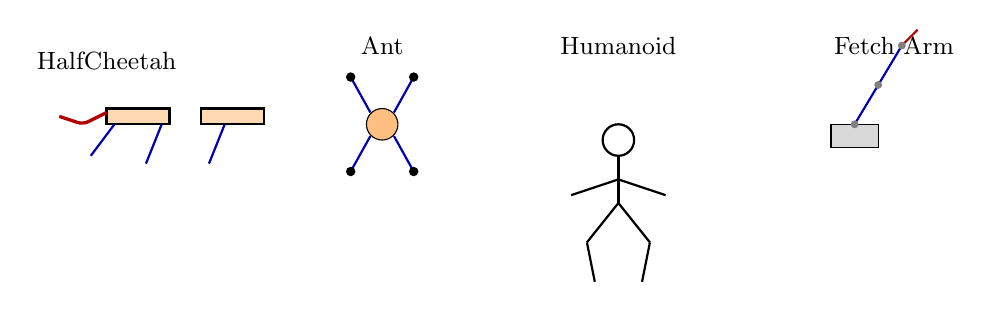
\begin{tikzpicture}[scale=1.0,>=stealth]
    % HalfCheetah (simplified)
    \begin{scope}[shift={(0,0)}]
        \node at (0,0.8) {\small HalfCheetah};
        \draw[thick,fill=orange!30] (0,0) rectangle (0.8,0.2); % body front
        \draw[thick,fill=orange!30] (1.2,0) rectangle (2.0,0.2); % body back
        \draw[very thick,red!70!black,rounded corners=2pt] (0,0.15) -- (-0.3,0) -- (-0.6,0.1); % head
        \draw[thick,blue!70!black] (0.1,0) -- (-0.2,-0.4); % front leg
        \draw[thick,blue!70!black] (0.7,0) -- (0.5,-0.5); % back leg
        \draw[thick,blue!70!black] (1.5,0) -- (1.3,-0.5); % back leg 2
    \end{scope}
    
    % Ant (simplified - top view)
    \begin{scope}[shift={(3.5,0)}]
        \node at (0,1.0) {\small Ant};
        \draw[fill=orange!50] (0,0) circle (0.2);
        \draw[thick,blue!70!black] (0.15,0.15) -- (0.4,0.6);
        \draw[thick,blue!70!black] (-0.15,0.15) -- (-0.4,0.6);
        \draw[thick,blue!70!black] (0.15,-0.15) -- (0.4,-0.6);
        \draw[thick,blue!70!black] (-0.15,-0.15) -- (-0.4,-0.6);
        \fill (0.4,0.6) circle (0.06);
        \fill (-0.4,0.6) circle (0.06);
        \fill (0.4,-0.6) circle (0.06);
        \fill (-0.4,-0.6) circle (0.06);
    \end{scope}
    
    % Humanoid (simple stick figure)
    \begin{scope}[shift={(6.5,-0.5)}]
        \node at (0,1.5) {\small Humanoid};
        \draw[thick] (0,0.3) circle (0.2); % head
        \draw[thick] (0,0.1) -- (0,-0.5); % torso
        \draw[thick] (0,-0.5) -- (-0.4,-1.0); % left leg
        \draw[thick] (-0.4,-1.0) -- (-0.3,-1.5); % left lower leg
        \draw[thick] (0,-0.5) -- (0.4,-1.0); % right leg
        \draw[thick] (0.4,-1.0) -- (0.3,-1.5); % right lower leg
        \draw[thick] (0,-0.2) -- (-0.6,-0.4); % left arm
        \draw[thick] (0,-0.2) -- (0.6,-0.4); % right arm
    \end{scope}
    
    % Fetch arm
    \begin{scope}[shift={(9.5,0)}]
        \node at (0.5,1.0) {\small Fetch Arm};
        \draw[fill=gray!30] (-0.3,0) rectangle (0.3,-0.3); % base
        \draw[thick,blue!70!black] (0,0) -- (0.3,0.5); % link 1
        \draw[thick,blue!70!black] (0.3,0.5) -- (0.6,1.0); % link 2
        \draw[thick,red!70!black] (0.6,1.0) -- (0.8,1.2); % gripper
        \fill[gray] (0,0) circle (0.05);
        \fill[gray] (0.3,0.5) circle (0.05);
        \fill[gray] (0.6,1.0) circle (0.05);
    \end{scope}
\end{tikzpicture}
\caption{常见机器人控制仿真环境示意图。从左到右依次为：HalfCheetah（2D猎豹行走）、Ant（四足机器人行走）、Humanoid（双足人形机器人行走）、Fetch Robot Arm（机械臂抓取）。这些环境涵盖了从较简单到极复杂的连续控制任务。}
\label{fig:envs}
\end{figure}

\section{经典控制任务}

本节详细介绍几个经典控制任务的数学表述，从入门级任务逐步过渡到复杂任务。

\subsection{CartPole（入门级）}

CartPole（倒立摆小车）是最经典的RL入门问题。任务目标是通过左右移动小车来保持上面的杆子竖直。

\textbf{状态}：$\states = [x, \dot{x}, \theta, \dot{\theta}]$，其中 $x$ 是小车的位置，$\theta$ 是杆子与竖直方向的夹角。

\textbf{动作}：向左或向右施加 $10\text{N}$ 的力（离散动作空间）或连续力（连续版本）。

\textbf{动力学}（连续版本）：
\begin{myformula}
\ddot{\theta} = \frac{g\sin\theta + \cos\theta\left(\frac{-F - m_p l \dot{\theta}^2 \sin\theta}{m_c + m_p}\right)}{l\left(\frac{4}{3} - \frac{m_p \cos^2\theta}{m_c + m_p}\right)}
\end{myformula}

其中 $m_c$ 为小车质量，$m_p$ 为杆质量，$l$ 为杆长的一半。

\subsection{HalfCheetah（中等难度）}

HalfCheetah 是二维平面内的"半猎豹"模型，只有前腿和后腿，任务是学会向前奔跑。

\textbf{状态}（17维）：包含躯干的 $z$ 坐标、角度、速度，以及各关节的角度和角速度。

\textbf{动作}（6维）：控制髋关节、膝关节等6个关节的力矩。

\textbf{奖励函数}：
\begin{myformula}
r_t = \dot{x}_{\text{torso}} - 0.1 \cdot \|\actions_t\|^2
\end{myformula}

即奖励前向速度同时惩罚大动作（能量消耗）。这一简练的奖励函数在HalfCheetah上效果极好——策略自然地学会了类似奔跑的步态。

\subsection{Ant（中等难度）}

Ant是四足机器人在三维空间中的行走任务。机器人有4条腿，每条腿有2个关节（8个关节总计）。

\textbf{状态}（27维）：包括躯干的位置、方向、线速度、角速度，以及各关节的状态。

\textbf{奖励函数}：
\begin{myformula}
r_t = \dot{x}_{\text{torso}} - 0.5 \cdot \|\actions_t\|^2 + 1.0 \quad\text{(存活奖励)}
\end{myformula}

Ant的挑战在于四条腿之间的协调——策略需要学会交替迈步来维持平衡和前进。

\subsection{Humanoid（困难级别）}

Humanoid是仿人双足机器人的行走任务，是 MuJoCo 中最具挑战性的标准任务之一。机器人有头部、躯干、两条手臂和两条腿。

\textbf{状态}（376维）：包含大量冗余信息（各刚体的位置、方向、速度等）。

\textbf{动作}（17维）：控制躯干与各肢体的关节力矩。

\textbf{关键挑战}：
\begin{itemize}
    \item 高维状态和动作空间导致探索困难
    \item 双足行走本身是不稳定的极限环，极易摔倒
    \item 手臂的动作可能与行走无关，策略需要学会抑制不必要的运动
    \item 训练通常需要 500万--2000万步才能获得可接受的行走策略
\end{itemize}

\begin{remark}
Humanoid是RL算法性能的"试金石"——如果一种新算法在Humanoid上显著优于基线，这是一个强有力的证据。PPO通常在Humanoid上需要约500万--1000万步，SAC稍快一些，而基于模型的RL方法（如Dreamer、TD-MPC）可以达到300万步以内。
\end{remark}

\subsection{Fetch Robot Arm（操作任务）}

Fetch环境模拟了一个7自由度机械臂，包含多个子任务：
\begin{itemize}
    \item \texttt{FetchReach-v2}：将末端执行器移到目标位置
    \item \texttt{FetchPush-v2}：推一个方块到目标位置
    \item \texttt{FetchPickAndPlace-v2}：抓取方块并放到目标位置
\end{itemize}

这些任务特别适合使用 Hindsight Experience Replay（HER，见第6节），因为在标准RL算法下，随机探索几乎不可能偶然完成"抓取-放置"这样的复杂操作。

\section{训练策略}

\subsection{PPO在MuJoCo上的超参数配置}

Proximal Policy Optimization（PPO，见第6章）是机器人RL中最常用的on-policy算法。以下是MuJoCo任务上的典型超参数配置：

\begin{table}[htbp]
\centering
\caption{PPO在MuJoCo上的推荐超参数}
\label{tab:ppo_hp}
\begin{tabular}{lc}
\toprule
超参数 & 典型值 \\
\midrule
学习率 & $3 \times 10^{-4}$ \\
批大小（总步数） & 2048 \\
小批大小 & 64 \\
优化轮数 & 10 \\
剪切参数 $\epsilon$ & 0.2 \\
折扣因子 $\gamma$ & 0.99 \\
GAE $\lambda$ & 0.95 \\
值函数系数 & 0.5 \\
熵系数 & 0.0--0.01 \\
最大梯度范数 & 0.5 \\
网络结构 & [64, 64] 全连接 + Tanh \\
激活函数 & Tanh（最后层线性） \\
并行环境数 & 1--64 \\
\bottomrule
\end{tabular}
\end{table}

\subsection{SAC在连续控制中的优势}

Soft Actor-Critic（SAC，见第6章）是off-policy算法，在连续控制任务中通常比PPO更样本效率高（但每步计算量更大）：

\begin{itemize}
    \item \textbf{自动熵调节}：SAC自动调整探索噪声的幅度，在不同训练阶段（初期多探索 vs 后期精细控制）自适应平衡exploration-exploitation
    \item \textbf{Off-policy效率}：在样本稀缺的场景中（如真实机器人的微调），SAC的样本效率优势很关键
    \item \textbf{多模态行为}：最大化熵的策略自然产生多样化行为，有利于探索
\end{itemize}

典型SAC超参数：
\begin{table}[htbp]
\centering
\caption{SAC在MuJoCo上的推荐超参数}
\label{tab:sac_hp}
\begin{tabular}{lc}
\toprule
超参数 & 典型值 \\
\midrule
学习率（Actor/Critic） & $3 \times 10^{-4}$ \\
目标平滑系数 $\tau$ & 0.005 \\
回放缓冲区大小 & $10^6$ \\
批大小 & 256 \\
折扣因子 $\gamma$ & 0.99 \\
网络结构 & [256, 256] 全连接 + ReLU \\
随机策略标准差范围 & $[-20, 2]$（经过tanh后） \\
每环境步的梯度步数 & 1 \\
初始随机步数 & 10000 \\
\bottomrule
\end{tabular}
\end{table}

\subsection{并行训练}

并行训练（Vectorized Environments）是加速RL训练的关键技术。基本思想是同时运行 $N$ 个独立的环境实例，收集 $N$ 倍的交互数据。

\begin{myalgorithm}{向量化环境训练框架}
\begin{enumerate}
    \item 创建 $N$ 个独立的环境副本
    \item 每个副本各自重置，获取初始状态
    \item 在每个训练迭代中：
    \begin{itemize}
        \item 对各副本的状态分别使用策略 $\pi_\theta$ 采样动作
        \item 所有副本并行执行 \texttt{step()}（可利用多核CPU或GPU）
        \item 收集各副本的 transition $(s, a, r, s')$
        \item 将收集到的数据传递给学习算法
    \end{itemize}
\end{enumerate}
\end{myalgorithm}

对于PPO，$N$ 个环境各收集 $T$ 步，总batch size为 $N \times T$。典型配置为 $N=64, T=2048$。

对于SAC等off-policy方法，并行化的主要好处是加速数据收集（填充回放缓冲区），而梯度更新在另一个线程中独立进行。

\begin{remark}
在GPU加速的仿真环境中（如 NVIDIA Isaac Gym），可以在单个GPU上同时仿真数千个机器人，每个环境独立运行但共享GPU的计算资源。这使得以前需要数周的训练任务可以在数小时内完成。极端情况下，Isaac Gym可以在RTX 3090 GPU上同时仿真4096个Ant环境，单日产生超过10亿步的交互数据。
\end{remark}

\subsection{训练曲线解读}

评估训练过程需要关注以下指标：

\begin{itemize}
    \item \textbf{回合平均奖励（Episode Reward Mean）}：最直接的性能指标，但可能被奖励成形误导
    \item \textbf{回合平均长度（Episode Length Mean）}：如果策略早早摔倒，回合会变短
    \item \textbf{值函数损失（Value Loss）}：反映价值估计的准确性
    \item \textbf{策略熵（Policy Entropy）}：反映策略的探索程度，持续下降表明策略在收敛
    \item \textbf{解释方差（Explained Variance）}：$\approx 1 - \frac{\text{Var}(R - V)}{\text{Var}(R)}$，衡量价值函数对实际回报的拟合程度
    \item \textbf{KL散度（Approx KL）}：PPO中策略更新的幅度，过大说明学习率过高
\end{itemize}

\subsection{常见问题与调试}

\begin{itemize}
    \item \textbf{策略不学习（奖励不增长）}
    \begin{itemize}
        \item 检查奖励尺度——过大的奖励会导致梯度爆炸
        \item 增大熵系数以提高探索
        \item 使用势函数成形提供密集信号
    \end{itemize}
    \item \textbf{策略过度振荡}
    \begin{itemize}
        \item 添加平滑性惩罚
        \item 降低学习率
        \item 在PPO中减小 $\epsilon$ 或增加优化轮数之间的KL早停
    \end{itemize}
    \item \textbf{Q值爆炸（SAC/TD3）}
    \begin{itemize}
        \item 降低学习率或增大目标网络软更新系数 $\tau$
        \item 使用梯度裁剪
        \item 检查回放缓冲区中是否存在极端奖励值
    \end{itemize}
    \item \textbf{PPO中KL散度过大}
    \begin{itemize}
        \item 降低学习率或减小 batch size
        \item 实施KL早停（当平均KL超过阈值时停止该epoch的更新）
    \end{itemize}
\end{itemize}

\section{进阶技术}

\subsection{Curriculum Learning}

Curriculum Learning（课程学习）的思想源自人类教育：从简单任务开始学习，逐步提高难度。在机器人RL中：

\begin{myalgorithm}{机器人RL的课程学习示例}
阶段1（简单的子任务）：
\begin{itemize}
    \item 行走任务：降低目标速度，增大摩擦以增加稳定性
    \item 操作任务：增大目标容差，从固定的初始位置开始
\end{itemize}

阶段2（中等难度）：
\begin{itemize}
    \item 行走任务：逐步提高目标速度
    \item 操作任务：逐步将初始位置随机化
\end{itemize}

阶段3（最终难度）：
\begin{itemize}
    \item 行走任务：在崎岖地形上行走
    \item 操作任务：减小目标容差到实际任务水平
\end{itemize}

课程策略在每一阶段训练收敛后自动进入下一阶段。
\end{myalgorithm}

\begin{figure}[htbp]
\centering
\begin{tikzpicture}[>=stealth, scale=0.9]
    % Three stages as boxes with increasing width
    \draw[thick,fill=green!10] (0,0) rectangle (3,1.5);
    \node at (1.5,0.75) [align=center] {\small 阶段 1：慢速行走\\{\footnotesize 目标速度 0.5 m/s}};
    
    \draw[->,thick] (3,0.75) -- (4,0.75);
    
    \draw[thick,fill=yellow!15] (4,0) rectangle (7.5,1.5);
    \node at (5.75,0.75) [align=center] {\small 阶段 2：正常行走\\{\footnotesize 目标速度 1.5 m/s}};
    
    \draw[->,thick] (7.5,0.75) -- (8.5,0.75);
    
    \draw[thick,fill=red!10] (8.5,0) rectangle (12.5,1.5);
    \node at (10.5,0.75) [align=center] {\small 阶段 3：崎岖地形奔跑\\{\footnotesize 目标速度 3.0 m/s}};
    
    % Annotations below
    \node at (1.5,-0.5) {\footnotesize 简单};
    \node at (5.75,-0.5) {\footnotesize 中等};
    \node at (10.5,-0.5) {\footnotesize 困难};
    
    % Arrow indicating progression
    \draw[->,thick,gray] (0,-1) -- (12.5,-1);
    \node at (6.25,-1.5) {\small 训练进程};
\end{tikzpicture}
\caption{课程学习进展示意。策略从简单的慢速行走开始训练，当在阶段1达到性能阈值时自动进入阶段2，依此类推。每个阶段使用前一阶段学到的策略作为初始化（warm start），显著加速了最终策略的收敛。}
\label{fig:curriculum}
\end{figure}

\subsection{多任务RL}

多任务强化学习（Multi-Task RL）训练一个策略同时掌握多个不同的技能。关键挑战是各任务之间可能相互干扰（negative transfer）。

常见的多任务RL方法包括：
\begin{itemize}
    \item \textbf{任务条件策略}：$\pi(\actions \mid \states, \mathbf{z})$，其中 $\mathbf{z}$ 是任务编码（one-hot向量或连续嵌入）
    \item \textbf{共享表示学习}：在多个任务之间共享网络底层特征，任务特定的头部负责不同行为
    \item \textbf{目标条件RL}：将任务目标直接作为状态的一部分（如目标位置），策略被训练为在条件化于不同目标时产生不同行为
\end{itemize}

\subsection{元学习（Meta-RL）}

元学习的目标是训练一个"学会学习"的策略，使其能够快速适应新任务。在机器人领域，这意味着：

\begin{itemize}
    \item \textbf{快速适应}：在新环境中只需少量交互（如5--50个episodes）就能学会新技能
    \item \textbf{稳健性}：对动力学参数的变化（如不同地面、不同有效载荷）具有快速适应能力
\end{itemize}

经典的Meta-RL方法包括MAML（Model-Agnostic Meta-Learning）和RL$^2$。MAML的核心理念是找到能在少量梯度步内快速适应新任务的初始策略参数。

\begin{myformula}
\theta^* = \arg\max_\theta \sum_{\mathcal{T}_i \sim p(\mathcal{T})} \E_{\tau \sim \pi_{\theta'_i}}\Big[\sum_t r_t^{\mathcal{T}_i}\Big]
\end{myformula}

其中 $\theta'_i = \theta + \alpha \nabla_\theta \E[\sum r]$ 是元梯度更新后的参数。这一元目标直接优化初始参数 $\theta$ 的快速适应能力。

\subsection{Hindsight Experience Replay (HER)}

HER 是解决稀疏奖励问题的经典方法，由 Andrychowicz 等人于2017年提出。其核心思想极为巧妙：\textbf{将失败当作成功来学习}。

\begin{mydefinition}{Hindsight Experience Replay}
对于一个以目标为导向的MDP（状态包含目标 $\states = [s_{\text{obs}}, g]$），假设策略的实际轨迹最终到达了某个状态 $s_{\text{final}}$（可能并非原始目标 $g$）。HER将这条失败轨迹"回头看"（in hindsight）重新标记为：目标不是 $g$，而是策略实际到达的 $s_{\text{final}}$，于是这条轨迹就变成了一条"成功"的轨迹。
\end{mydefinition}

\begin{myalgorithm}{HER 算法}
\textbf{输入}：off-policy RL算法 $\mathcal{A}$（如DDPG、SAC），采样策略 $\pi$，重放比例 $k$

\textbf{对于每个 episode}：
\begin{enumerate}
    \item 采样目标 $g$ 和初始状态 $s_0$
    \item 使用策略 $\pi$ 执行 rollout，获得轨迹 $(s_0, a_0, r_0, s_1, \ldots, s_T)$。注意：状态中包含了原始目标 $g$，奖励函数 $r(s, a, g)$ 是基于 $g$ 计算的。
    \item 将原始轨迹存储到回放缓冲区
    \item 对于 $m = 1, \ldots, k$：
    \begin{itemize}
        \item 采样一个 hindsight 目标 $g'$（通常从本轨迹的某个未来状态中选择）
        \item 对轨迹中每个 transition $(s_t, a_t, r_t, s_{t+1})$：
        \begin{itemize}
            \item 用 $g'$ 替换 $s_t$ 和 $s_{t+1}$ 中的目标部分
            \item 重新计算奖励 $r_t' = r(s_t, a_t, g')$
            \item 将重新标记的 transition 存入缓冲区
        \end{itemize}
    \end{itemize}
    \item 使用算法 $\mathcal{A}$ 更新策略
\end{enumerate}
\end{myalgorithm}

\begin{myTheorem}{HER的探索效率}
对于 $N$ 维连续目标的抓取任务，随机探索首次偶然成功的概率在指数级上趋近于0（对于如 $\pm 1\text{cm}$ 的容差，成功率 $\propto (0.02)^3 = 8\times 10^{-6}$）。HER将每条轨迹转化为 $k+1$ 条"成功"示范，使得即使从未真正成功的策略也能从失败中学到"如何到达某些状态"。
\end{myTheorem}

HER在Fetch Robot Arm系列任务中取得了突破性成果——特别是在FetchPickAndPlace这样的复杂任务中，标准的DDPG几乎完全无法学习，而DDPG+HER可以稳定地解决这些任务。

\begin{figure}[htbp]
\centering
\begin{tikzpicture}[>=stealth, scale=1.0]
    % Trajectory visualization
    \draw[->] (0,0) -- (8,0) node[right]{时间};
    \draw[->] (0,0) -- (0,4) node[above]{$y$};
    
    % Actual trajectory
    \draw[thick,blue!70!black,->] (0,0.5) .. controls (2,1.5) and (4,2.5) .. (6,3.0) .. controls (7,3.2) .. (7.5,3.5);
    
    % Goal markers
    \fill[red] (7.8,0.3) circle (0.1) node[right]{原始目标 $g$};
    \fill[green!60!black] (7.5,3.5) circle (0.1) node[right]{实际到达};
    
    % Hindsight relabel
    \draw[->,dashed,green!60!black,thick] (6,1.5) .. controls (6.5,2) .. (7.5,3.5);
    \node[green!60!black] at (6.5,1.0) {重新标记为成功轨迹};
    
    % States along trajectory
    \foreach \x/\y in {1/0.8, 2/1.3, 3/1.8, 4/2.2, 5/2.6} {
        \fill (\x,\y) circle (0.06);
    }
    \fill (7.5,3.5) circle (0.08);
    
    % Annotation
    \node[align=left,text width=4cm] at (3,-1) {原轨迹以 $g$ 为目标：\\全程奖励 = 0（失败）};
    \node[align=left,text width=4cm] at (3,-2) {Hindsight重标记以 $g'=s_{\text{final}}$ 为目标：\\后几步成功到达！};
\end{tikzpicture}
\caption{HER hindsight重标记示意。蓝色实线是策略的实际运动轨迹，红色点是原始目标（策略未能到达），绿色点是策略实际到达的状态。在hindsight重标记中，我们将轨迹的目标替换为策略实际到达的位置，从而将"失败"转化为"成功"的示范数据。}
\label{fig:her}
\end{figure}

\section{真实机器人部署的挑战}

从仿真中训练好的策略部署到真实机器人上，面临着一系列挑战，这些挑战将在第12章中被深入探讨。本节简要概述：

\subsection{执行器延迟}

真实电机的响应不是瞬时的。从发出指令到执行器实际产生力矩之间存在延迟（通常 1--20ms），这在高速运动中影响显著。延迟主要来源于：
\begin{itemize}
    \item 通信延迟（控制器到电机驱动器的信号传输）
    \item 机械惯性延迟
    \item 电流环响应时间
\end{itemize}

在仿真中加入延迟建模是提高策略可迁移性的重要手段。

\subsection{传感器噪声}

真实传感器的测量带有噪声，包括：
\begin{itemize}
    \item \textbf{编码器量化噪声}：位置测量存在有限的离散精度
    \item \textbf{IMU漂移}：角速度积分导致姿态估计漂移
    \item \textbf{力/力矩传感器噪声}：通常呈高斯分布但有频率依赖性
\end{itemize}

策略需要在噪声环境中保持稳健性，这可以通过在训练时向状态注入噪声来实现。

\subsection{安全约束}

真实机器人上，摔倒或碰撞可能导致昂贵的硬件损坏。安全措施包括：
\begin{itemize}
    \item 关节力矩限制（硬件层面由电机驱动器实现）
    \item 关节位置/速度软件限位
    \item 紧急停止按钮和碰撞检测
    \item 在外部安全控制器中进行动作合法性验证
\end{itemize}

\subsection{实时性要求}

RL策略的推理必须在控制周期内完成。对于 100Hz 的控制频率，策略的前向传播必须在 10ms 内完成。这对网络架构设计提出了限制——不能使用过于庞大的模型。此外，操作系统层面的实时性能也需要保障（使用实时操作系统或实时内核补丁）。

\begin{remark}
从仿真成功到真实部署成功之间存在一个著名的"Sim-to-Real Gap"（仿真-真实鸿沟），它需要专门的应对策略——域随机化、系统辨识、域自适应等技术。这些内容构成了第12章的核心议题。
\end{remark}

\section{本章小结}

本章系统介绍了强化学习在机器人控制中的应用方法论。我们从将机器人控制问题转换为MDP入手，讨论了状态空间和动作空间的设计，以及如何将复杂的动力学方程融入RL框架。奖励函数设计是机器人RL最核心的工程挑战——从目标导向到势函数成形，从稀疏奖励的困境到HER的创新解决方案。我们介绍了主流的仿真环境和训练策略，包括PPO和SAC在连续控制任务中的实战配置和调优技巧。最后概述了真实机器人部署面临的挑战，为下一章的深度讨论做了铺垫。

% --- END OF CHAPTER 11 ---
